\documentclass[conference]{IEEEtran}
\usepackage[utf8]{inputenc}
\usepackage{amsfonts}
\usepackage{caption}
\usepackage{graphicx}
\usepackage{listings}
\lstset{
    basicstyle=\tiny\ttfamily,
    keywordstyle=\color{blue}\ttfamily,
    stringstyle=\color{red}\ttfamily,
    commentstyle=\color{green}\ttfamily,
    breaklines=true
}
\usepackage{url}

% correct bad hyphenation here
\hyphenation{op-tical net-works semi-conduc-tor}

\begin{document}
\title{Relatório - EP3}

\author{\IEEEauthorblockN{Tiago Koji Castro Shibata - 8988730}
\IEEEauthorblockA{Escola Politécnica\\
Universidade de São Paulo\\
tiago.shibata@usp.br}
}

\maketitle

\section{Introdução}
Esse relatório acompanha o terceiro exercício programa (EP3) da disciplina PCS3556 - Lógica Computacional.

\hfill 26 de Março de 2018

\section{Tarefa}

A tarefa consiste em implementar um algoritmo de ... O algoritmo deve retornar se ...

\section{Algoritmo}

O algoritmo deve suportar ... (ou seja, pela hierarquia de Chomsky, ...):
\\
\\
\begin{minipage}{\linewidth}
    \centering
    \label{chomsky}
    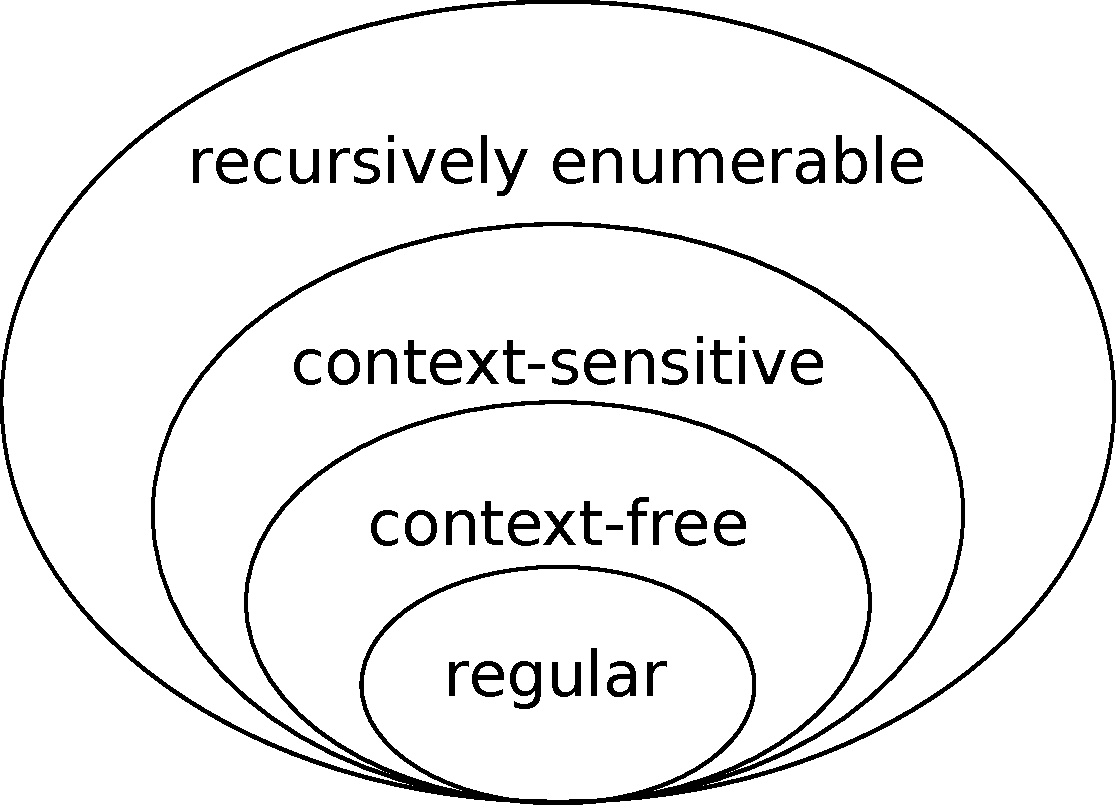
\includegraphics[width=0.8\textwidth]{Chomsky-hierarchy.pdf}
    \captionof{figure}{Hierarquia de Chomsky}
\end{minipage}

Conforme especifiado, a implementação é recursiva e feita em Elixir, uma linguagem funcional. Conforme sugerido no enunciado, ...

\section{Estruturas de dados}

Em alguns locais, estruturas de conjunto fornecidas pelo Elixir ($MapSet$) foram usadas tendo em mente performance e facilidade: o uso de conjunto evita que varramos a lista toda para buscar um elemento, e o conjunto permite operações fáceis e rápidas de união ou diferença quando necessário.

\section{Código e testes}

A função $example(arg1, arg2)$ recebe uma ... Ela gera ...

A regra é dada como uma tupla $\{cadeia\ inicial, cadeia\ a\ ser\ colocada\}$. Foram escritos testes para essa função:

% \lstinputlisting{1_test.ex}

Os testes foram essenciais no desenvolvimento, já que essa função apresenta muitos \emph{corner cases}. Por exemplo, ...

A função foi implementada buscando a primeira correspondência da condição da regra na forma sentencial com a função \emph{String.split}...:

% \lstinputlisting{1.ex}

\begin{thebibliography}{1}
\bibitem{elixir}
Friedel Ziegelmayer. \emph{Elixir ExDoc}. \url{https://hexdocs.pm/elixir/}, acessado em 11/02/2018
\end{thebibliography}

\end{document}
